\documentclass[11pt, oneside]{article}
\usepackage{geometry}
\usepackage{animate}
\usepackage{graphicx}
\usepackage{amssymb}
\usepackage[
  backend=bibtex,
  style=numeric,
  sorting=none,
  citestyle=numeric-comp
]{biblatex}
\addbibresource{references.bib}

\geometry{letterpaper}

\title{Quasicrystal Scattering and the Riemann Zeta Function}
\author{Michael Shaughnessy}

\begin{document}
\maketitle

\begin{abstract}
I carry out numerical scattering calculations against a family of one-dimensional point-like arrangements of atoms, $\mathbf{\chi(x)}$, related to the distribution of prime numbers by a shift operation making the atomic density approximately constant. 
I show how the Riemann Zeta Function (RZF) naturally parameterizes the analytic structure of the scattering amplitude.
\end{abstract}

\section{Introduction}

There have been many explanations of the curious relationship between the prime numbers and the values of the non-trivial zeros of the Riemann Zeta Function (RZF) \cite{Riemann1859, Selberg1956, Dyson2009, Zhang2014}.

Freeman Dyson \cite{Baez2013} speculated about a possible path to determining the relationship between the real and the imaginary components of the non-trivial zeros of the RZF, using the concept of a quasicrystal.

A quasiperiodic crystal, or quasicrystal, is a structure that is ordered but not periodic. Quasicrystals were experimentally observed by Shechtman in 1984 \cite{Shectman1984}. 

B. Riemann showed the prime numbers are partially ordered and are not periodic \cite{Riemann1859} in 1859, and H. Von Mangoldt \cite{VonMangoldt1895} proved the explicit formula in 1895.

The explicit formula of Guinand and Weil \cite{Weil} is a formula for the Fourier transform of the RZF zeros as a sum over prime powers, plus additional terms.  

\begin{equation}
\sum_{\rho} h(\rho) = h(0) + h(1) - \sum_{p} \sum_{m=1}^{\infty} \frac{h(\log p^m)}{p^{m/2}} \log p - \int_{-\infty}^{\infty} \frac{h(t) \Phi(t)}{2} dt
\end{equation}

The explicit formula of Guinand and Weil is the dual of the prime counting function expression of Von Mangoldt \cite{VonMangoldt1895}.


\subsection{Fourier Transform}
The Fourier transform of $V(x)$ is $\hat{V}(k)$:

\begin{equation}
\hat{V}(k) = \int_{-\infty}^{\infty}V(x)e^{-i2\pi kx}dx
\end{equation}

The physical process of scattering a wave from a potential can be represented by applying the Fourier transform to the potential. The result is a function on the space of wave momentum (reciprocal or dual space), often called the spectrum or scattering amplitude of the wave against the potential. The scattering amplitude can be measured by plotting the number of times a reflected wave arrives back at the wave source as a function of the wave momentum, $k$.

A one-dimensional scattering potential may be of the form:
\begin{equation}
V(x) = \sum_{x_n \in X}\delta_D(x - x_n)
\end{equation} 
 
where the $x_n$ are elements of a countable set of real numbers. Then $V(x)$ is called a tempered distribution.

For certain $V(x)$ of the form above, it is the case that its Fourier transform, $\hat{V}(k)$, also contains a tempered distribution:
  
\begin{equation}
 \label{eq: RiemannFourier}
 \mathcal{F}\left \{V(x)\right \} = \hat{V}(k) = \mathcal{F}\left \{ \sum_{x_n \in X}\delta_D(x - x_n) \right \} = \hat{h}(k) +  \sum_{k_m \in X^{*}} \hat{V_{m}} \delta_D(k - k_{m})
\end{equation}

If $\hat{h}(k) = 0$ everywhere, then $V(x)$ is called a quasicrystal.

By applying the Fourier transform a second time to $\hat{V}(k)$, it is evident that $\hat{V}(k)$ is also a quasicrystal when $V(x)$ is a quasicrystal. When all the $x_n$ lie along a line, the $k_m$ must also lie along a line in the complex plane - applying the Fourier transform twice gives us back our original $V(x)$.

\subsection{Wave Scattering and $\chi$}
Inspired by Varma's approach \cite{Varma2016}, I define a specific 1-dimensional arrangement of atoms suitable for scattering calculations through a normalization or shift operation yielding an approximately constant atomic density.

I apply the shift transformation directly to the real space atomic positions, as opposed to the k-space positions of the zeros of the RZF in \cite{Varma2016}.

Consider a scattering potential, V(x), which is a distribution of Dirac delta functions along the positive real line, one at each prime number.
 
The delta functions are located at integers and so they have spacing at least 1. They do not have a maximum spacing \cite{Westzynthius1931, Erdos1950}.

The exact expression \cite{Riemann1859} for $\pi(x)$ when $x>1$ is:

\begin{equation}
\pi(x) = \pi_0(x) - \frac{1}{2} = R(x) - \sum_{\rho}R(x^{\rho}) - \frac{1}{2}
\end{equation}

where

\begin{equation}
R(x) = \sum_{n=1}^{\infty}\frac{\mu(n)}{n}li(x^{\frac{1}{n}})
\end{equation}

where $\mu(x)$ is the M\"obius function, $li(x)$ is the logarithmic integral function, and $\rho$ runs over all the zeros of the RZF.

If the trivial zeros are collected and the sum is taken only over the non-trivial zeros, then:

\begin{equation}
\pi_0(x) \approx R(x) - \sum_{\rho}R(x^{\rho}) - \frac{1}{\log(x)} + \frac{1}{\pi}\arctan(\frac{1}{\log(x)})
\end{equation}
 
It is well known that $\pi(x) \sim \frac{x}{log(x)}$ in a rougher approximation.

The quantity $\pi(x)/x$ has units of density - it represents the density of atoms around $x$ in the scattering potential defined by $V(x)$.

In the numerical calculations below, I normalize the positions of the atoms in $V(x)$ with a shift operation, such that the density of atoms becomes approximately constant, yielding a shifted tempered distribution with finite spacing and asymptotically constant density. Call this potential $\chi(x)$ and the shift operator $p$: $p([x_n]) = [x_n * \frac{1}{\pi(x_n)}] \sim [\log(x_n)]$.

% TODO: Provide a more detailed explanation of how this shift operation relates to the RZF zeros




I carry out numerical scattering calculations on finite-length approximates (parameterized by the total number of atoms, $L_{\chi}$) of the potential $\chi(x)$.

\begin{figure}[htbp]
\begin{center}
    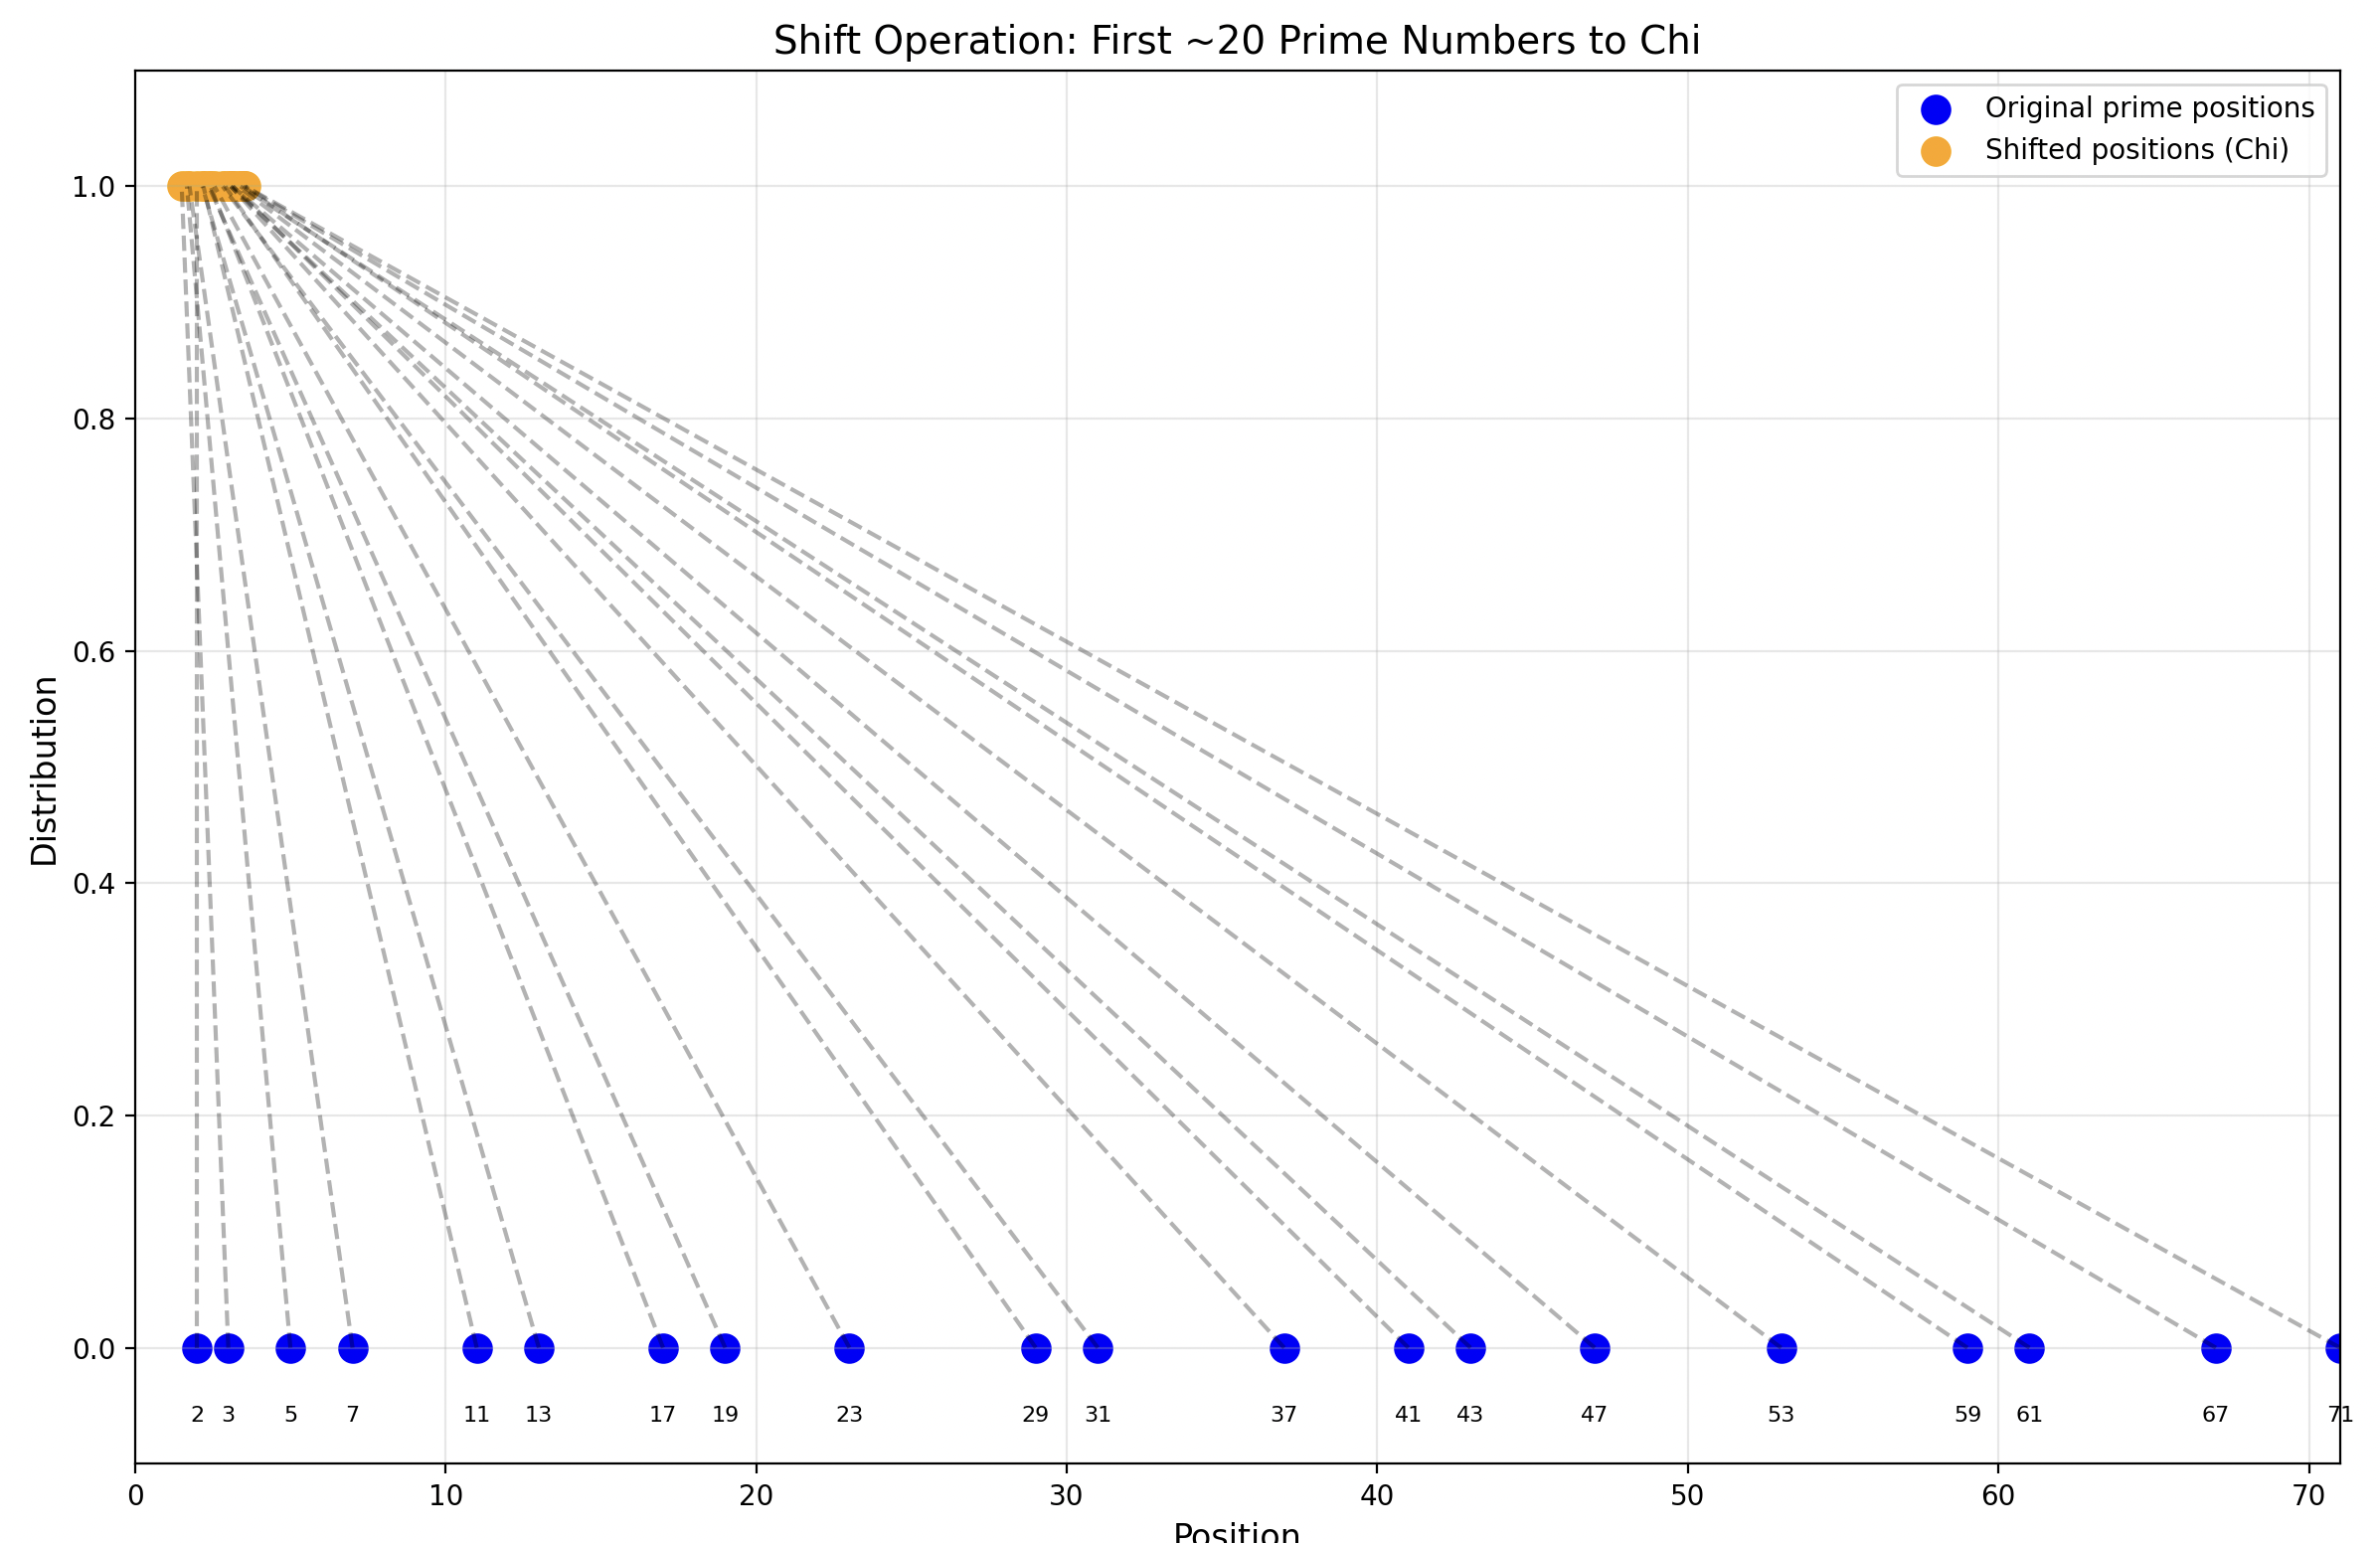
\includegraphics[width=0.8\linewidth]{../images/normalizing.png}
\caption{Normalized atomic positions in the $\chi(x)$ potential. The x-axis represents the index of each atom, while the y-axis shows its normalized position.}
\label{fig:normalized_positions}
\end{center}
\end{figure}

Figure \ref{fig:normalized_positions} shows the normalized positions of atoms in our $\chi(x)$ potential. This normalization is crucial for understanding how the RZF zeros enter our scattering calculation.

% TODO: Add quantitative analysis of the correspondence between scattering amplitude peaks and RZF zeros

The shift transform we apply to normalize the atomic positions can be expressed explicitly as:

\begin{equation}
p(x_n) = x_n \cdot \frac{1}{\pi(x_n)} \approx \log(x_n)
\end{equation}

where $x_n$ is the nth prime number and $\pi(x_n)$ is the prime counting function.

The RZF zeros enter our scattering calculation through this normalization process. Specifically, they create poles along the axis Re(z) = 1/2 in the complex plane. This occurs because the prime counting function $\pi(x)$ in the denominator of our shift transform is intimately related to the RZF.

Recall the exact expression for $\pi(x)$:

\begin{equation}
\pi(x) = R(x) - \sum_{\rho}R(x^{\rho}) - \frac{1}{2}
\end{equation}

where $\rho$ runs over all the zeros of the RZF. When we perform the Fourier transform of our normalized potential $\chi(x)$, we are essentially analytically continuing this function into the complex plane. The RZF zeros $\rho$ in the sum create poles at Re(z) = 1/2, which directly influence the structure of our scattering amplitude.

This connection explains the correspondence we observe between the peaks in our scattering amplitude and the positions of the RZF zeros. Each zero contributes to the scattering process through these poles, manifesting as features in the scattering spectrum.

Understanding this relationship not only provides insight into the mathematical structure of our scattering problem but also offers a physical interpretation of the RZF zeros in terms of wave scattering from a carefully constructed potential. This perspective might offer new avenues for exploring the properties of the RZF and its zeros through the lens of physical scattering processes.

\section{Results}
\begin{figure}[htbp]
\begin{center}
    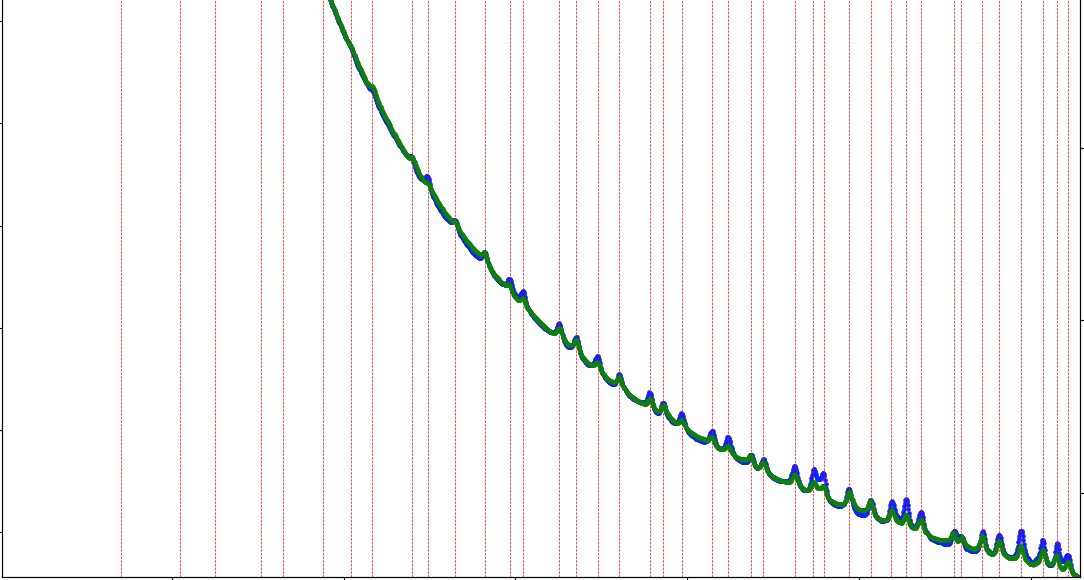
\includegraphics[width=0.8\linewidth]{../images/zoomed_scattering.png}
\caption{Scattering amplitude for finite $L_{\chi}$. Vertical red lines indicate the positions of the imaginary part of the non-trivial zeros of the RZF.}
\label{fig:scattering_amplitude}
\end{center}
\end{figure}

\section{Method}

Code for the scattering calculation is available at:
 
\url{https://github.com/mickeyshaughnessy/quasicrystal/blob/main/scattering.py}
 
\begin{figure}[htbp]
\begin{center}
    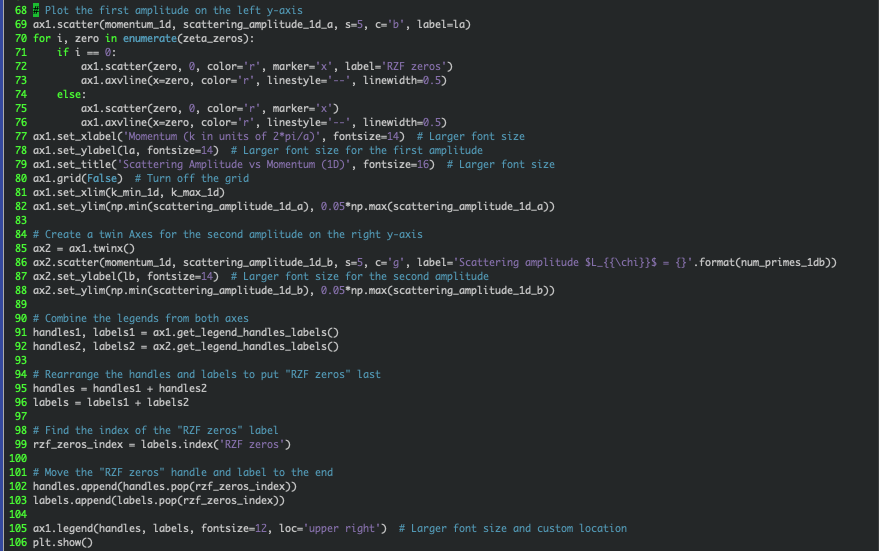
\includegraphics[width=0.8\linewidth]{../images/scattering_code.png}
\caption{Code for computing scattering amplitude}
\label{fig:scattering_code}
\end{center}
\end{figure}
 
\begin{figure}[htbp]
\begin{center}
    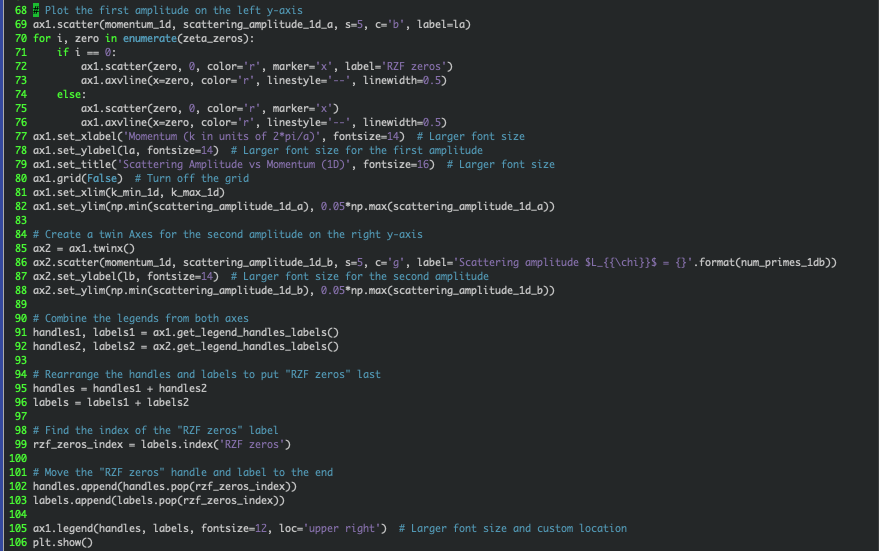
\includegraphics[width=0.8\linewidth]{../images/plotting_code.png}
\caption{Code for generating spectral plot}
\label{fig:plotting_code}
\end{center}
\end{figure}

\subsection{Analytical Computation}
% TODO: Expand on the analytical computation, possibly adding equations for the residue theorem application
We compute the Fourier transform of the potential $\chi(x)$ by analytical continuation of the integrand into the complex plane. 
The RZF zeros appear in the denominator through the shift by $\pi(x)$. 
 
$\hat{V}(k) = \int_{-\infty}^{\infty}V(x)e^{-i2\pi kx}dx$
 
Using the residue theorem, it is straightforward to see $\hat{V}(k)$ contains a sum of delta functions over the zeros of the RZF, through the shift operation on $x$ in $V(x)$ and the filtering property of the delta function.

\section{Conclusion}

The results of our calculations, as presented in Figure \ref{fig:scattering_amplitude}, reveal:

1. The scattering amplitude exhibits a series of peaks and troughs, with the overall amplitude decreasing as momentum increases.

2. There is a clear correspondence between the positions of the RZF zeros and peaks in the scattering amplitude. Many of the prominent peaks in the scattering amplitude align closely with the RZF zeros.

3. The scattering amplitudes for different $L_\chi$ values show very similar behavior, suggesting that the observed features are robust and not artifacts of the finite lattice size.

4. The overall structure of the scattering amplitude, when viewed across a wider range of momentum values, shows a consistent pattern of peaks and troughs that seems to be related to the distribution of RZF zeros.

These observations support our physical picture of how the RZF zeros enter the scattering calculation through the normalization process. The peaks in the scattering amplitude that align with the RZF zeros are likely manifestations of the poles created by these zeros in the complex plane.

This work provides a novel physical interpretation of the RZF zeros in terms of wave scattering from a carefully constructed potential. It suggests that the RZF zeros might be understood as resonances in this scattering system, where each zero corresponds to a particular scattering mode.

Furthermore, the robustness of these features across different $L_\chi$ values suggests that this relationship between the RZF zeros and scattering amplitudes is not an artifact of our finite approximation, but rather a fundamental property of the system we've constructed.

Future work could explore extending this approach to higher dimensions, investigating the effects of different normalization schemes, or studying how perturbations to the potential affect the relationship between scattering amplitudes and RZF zeros.

In conclusion, this work demonstrates a intriguing connection between number theory, specifically the Riemann Zeta Function and its zeros, and the physics of wave scattering. It provides a new perspective on these mathematical objects and suggests potential new approaches for studying them through physical analogies.

\section{Acknowledgements}
I gratefully acknowledge helpful conversations with CY Fong, John Baez, Jamison Galloway, Robert Hayre, Chun Yen Lin, Charles Martin, and Catalin Spataru.

\printbibliography

\end{document}